\newpage

\section{Author contributions}
\label{sec:authors}
All authors contributed to writing.
\begin{itemize}[leftmargin=*]
    \item Meera Hahn (meerahahn@google.com): Led automated evaluation and human evaluation of agents. Created DesignBench. Contributed to agent design and development.
    \item Wenjun Zeng (wenjunzeng@google.com): Significant contribution to agent design and development, as well as open-sourcing.
    \item Nithish Kannen (nitkan@google.com): Significant contribution to experiments and early versions of agents. Led open-sourcing.
    \item Rich Galt (richgalt@google.com): Led agent interface design and human studies.
    \item Kartikeya Badola (kbadola@google.com): Contributed to experiments and early versions of agents.
    \item Been Kim (beenkim@google.com): Advised project direction with critical feedback.
    \item Zi Wang (wangzi@google.com): Proposed and initiated project. Led agent design and development. Advised project. Contributed to evaluation.
\end{itemize}







\section{Novelty and contributions}
\label{app:novelty}
In this section, we emphasize the novelty and contributions of this work.

\begin{enumerate}
    \item System design of proactive T2I agents.
    \begin{itemize}
        \item Novel human-agent interaction modalities: Prior to our work, human users typically interact with current T2I systems by giving additional instructions or refining the prompt. To the best of our knowledge, our work is the first to propose a proactive T2I agent system that is able to ask clarification questions and present its belief graph for the user to edit.
\item Novel human-agent interaction interface:  We designed a new interface to best enable the clarification and belief graph interaction modalities. We have not seen these features in any T2I, or other generative media apps that are publicly live to date, signifying to us total uniqueness. Our human studies showed that at least 85\% of raters found each component of the interface useful for their workflow, for us proving that these are both novel and useful.
\item Novel design of different T2I agents that enable the proposed interaction modalities. Please see \S\ref{sec:blueprints} for the full details of the design principles and construction of those T2I agent prototypes (Ag1, Ag2, Ag3).
    \end{itemize}
    \item Our belief graphs significantly differs from classic belief states in the following ways:
    \begin{itemize}
        \item Hardcoded predicates v.s. Automatically-generated predicates: Traditionally, constructing classic symbolic belief states requires a pre-defined set of predicates such as “on(a, b)”, “is\_red(a)”, “at\_position(robot, x, y, z)” and it is non-trivial to learn new predicates that can be used and generalized to new tasks~\citep{pasula2007learning, xia2019}. Typically the pre-defined set of predicates are written by system developers and hardcoded into classic AI systems~\citep{fikes1971strips}. 
Our belief graphs do not require any pre-defined predicates. Instead, we propose to construct symbolic beliefs using a sequential in-context learning (ICL) method with LLMs (\Cref{alg:beliefparsing}). 
Our method can be generalized across a wide range of T2I tasks and achieve high performance (see our comprehensive results on Coco, Imageinwords, DesignBench). 
\item Applications: To the best of our knowledge, classic symbolic beliefs are mostly used for robot planning, and we are the first to use symbolic belief graphs to assist T2I tasks.

\item Data structure: Because of the application to planning, a symbolic world state is usually implemented and stored as a set or list of literals, i.e., atoms or negation of atoms where atoms are instantiated predicates~\citep{alkhazraji-et-al-zenodo2020,garrett2020pddlstream,garrett2020online}, so that whenever an action is applied, the agent can apply transition by adding and deleting items in the set according to the precondition and effect of the action. 

For T2I tasks, it is more convenient to use a graph to represent the world state associated with an image, since entities and relations naturally form a set of nodes (entities) and edges (relations between entities). Each component of the graph can also have probabilities, making it easy to turn a world state into a belief state using the same data structure. Hence we represent T2I agent beliefs using graphs. The agent can directly update the graph for each transition instead of going through a set or list.
\item Interpretability and controllability: The graph structure makes our agent belief more interpretable than traditional belief states, since we can visualize and progressively disclose the graph to the human user. Moreover, each node or relation in the belief graph has associated descriptions, making it easy for the user to understand and potentially edit every component of the belief graph. In our human studies, about 85\% of raters found the belief graph useful. To the best of our knowledge, our work is the first to use the graph-based belief state for human-AI interaction.
    \end{itemize}
    \item Automated evaluation of T2I agents: We propose a novel automated evaluation approach for T2I agents using self-play. The agent interacts with a simulated user that has access to the original image and its long caption. See \S\ref{ssec:automatic_eval} and \S\ref{ssec:user_simulation} for the full details of how the simulated user is constructed. This evaluation pipeline is easy to use and can help the future development of T2I agents.
\item DesignBench: We envision that a significant fraction of T2I users are artists and designers, and it is important to ensure that T2I agents are evaluated for these use cases. Hence we create DesignBench, featuring photo-realism, animation and multiple styles with short and long captions. DesignBench can be directly plugged into our automated evaluation to streamline the evaluation process.
\end{enumerate}


\section{Formalism of the agent and its objective} 

\label{ssec:objective}

We define an interactive T2I agent as a $\langle B, A, O, \tau, \pi\rangle$ tuple, where we have %

\begin{itemize}
    \item $S$: a representation space of images, %
    \item $B$: a space of agent beliefs, %
    \item $A$: a space of actions that the agent can take,
    \item $O$: a space of agent observations of the user,
    \item transition function $\tau: B\times A \times O\mapsto B$ for updating beliefs given new interactions,
    \item action selection strategy $\pi: B \mapsto A$, which specifies which action to take given a belief.
\end{itemize}

For each user-initiated interaction, we assume that there exists a specific intent $s\in S$, where $S$ is the space of all possible user intents. For a T2I task, we assume that the intent is the image the user would like to generate, and the intent stays the same throughout the interaction with an agent. We discuss more about the validity of this assumption in \S\ref{sec:discussion}.

Each type of T2I agents can have a unique user intent representation, belief representation, construction of the action space, and user interface design to obtain observations of users. %

In \S\ref{sec:blueprints}, we show the examples for these components.

We use a score function, $f: B\times S\mapsto \R$, to evaluate the alignment between an agent belief and a user intent at any turn of the interaction. Function $f$ can only be evaluated in hindsight once the user intent is revealed. The agent does not have direct access to function $f$ since the user intent is hidden from the agent. However, the agent may construct a probabilistic distribution over function $f$ based on its belief about the user intent. The goal of the agent is to maximize function $f$ with as few turns of interaction with the user as possible. 




\section{Visualization of Multi-Turn Agent-User Dialogs and Generated Images}
In \Cref{fig:dialog}, we show examples of multi-turn dialogs between simulated users and the three agents in \Cref{sec:exp}. We also visualize the generated images in \Cref{fig:toy1}, \Cref{fig:toy2}, \Cref{fig:coco1} and \Cref{fig:coco2}.
\begin{figure}
    \centering
    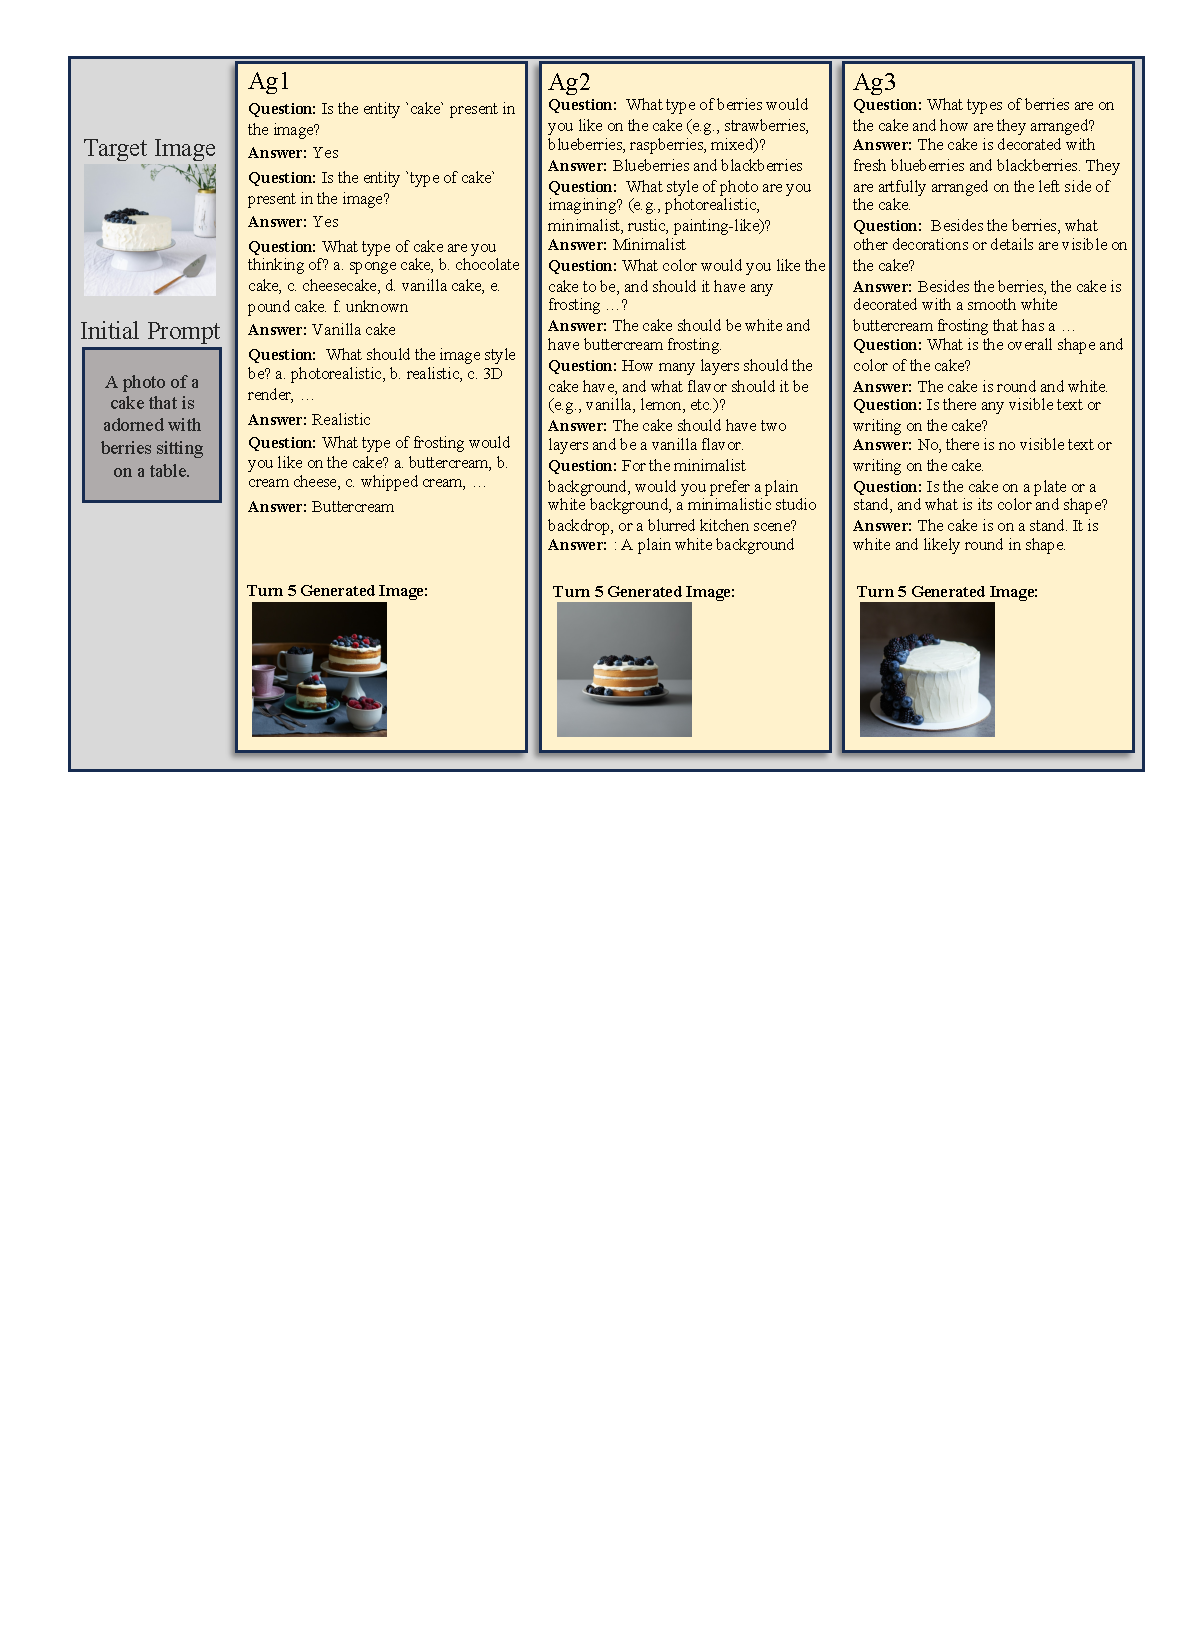
\includegraphics[width=\linewidth]{figures/dialog.pdf}
    \caption{Real multi-turn dialogs generated by the Ag1, Ag2, and Ag3 agents on an image from DesignBench. The figure additionally shows the image generated after the 5 turn dialog per agent.}
    \label{fig:dialog}
\end{figure}

\begin{figure}
    \centering
    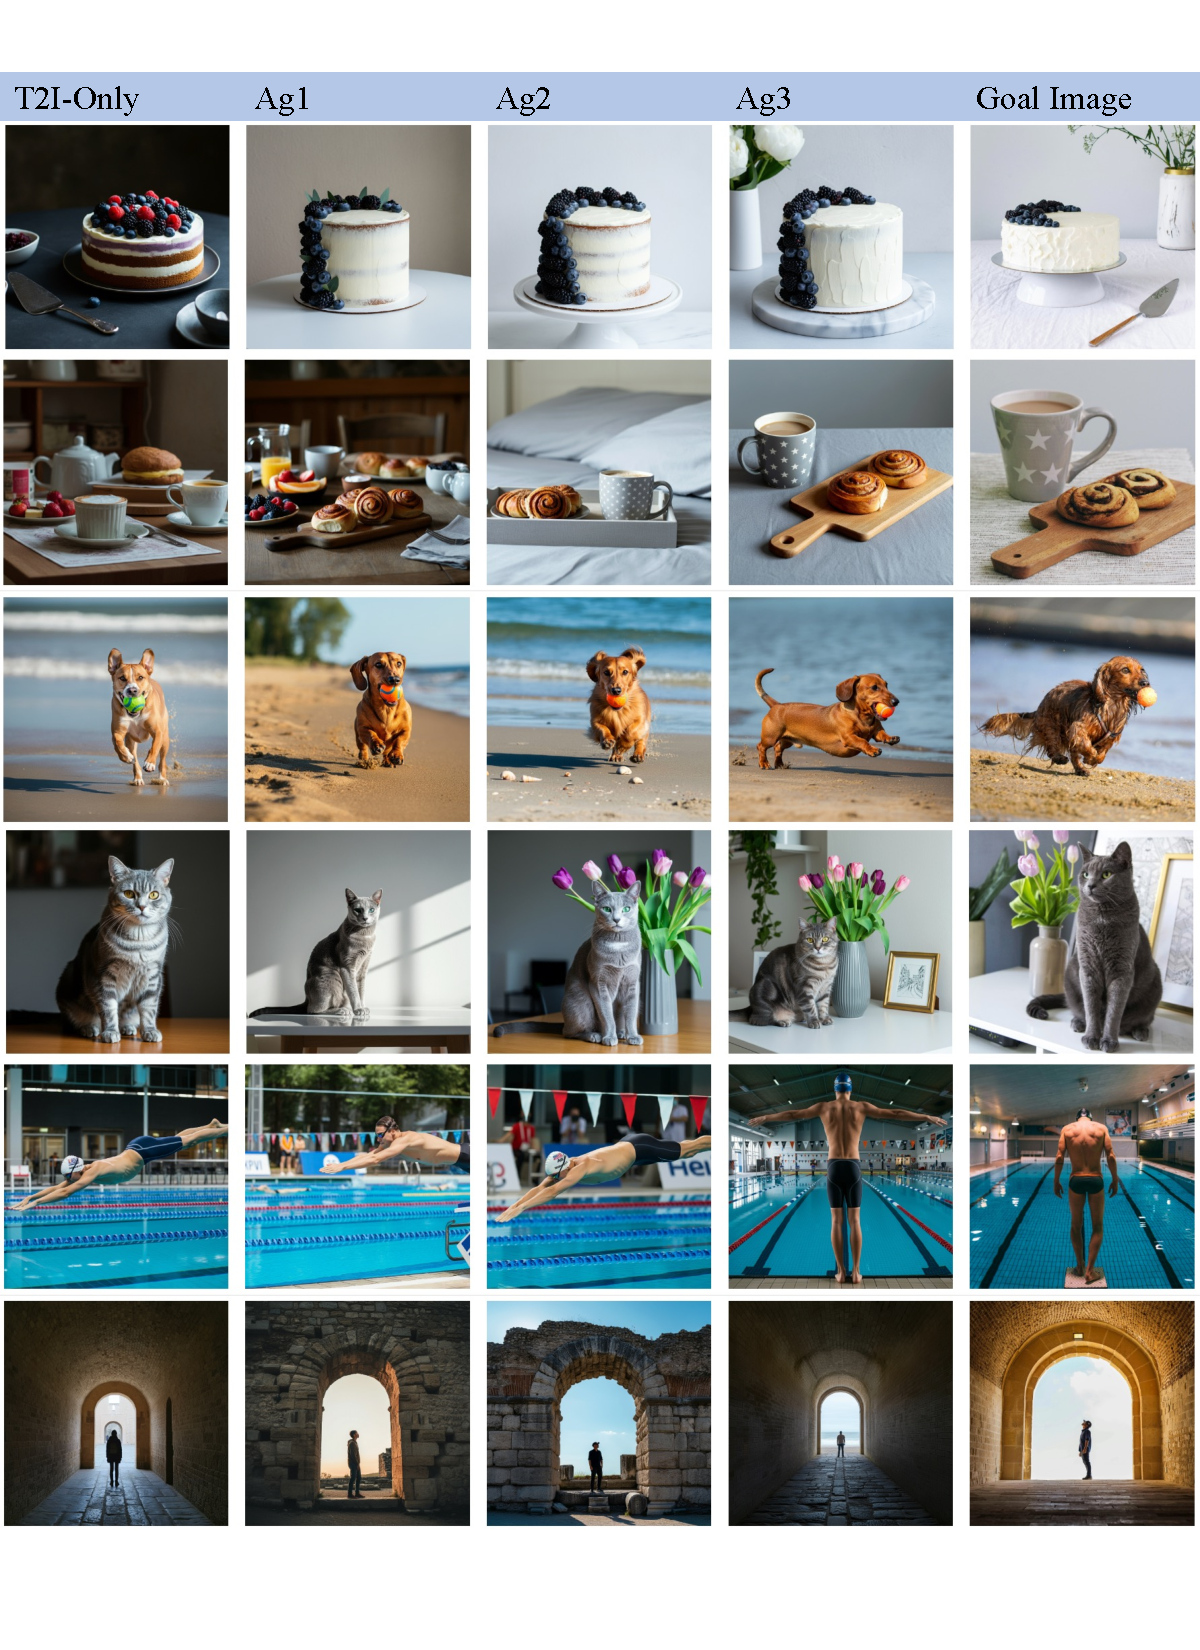
\includegraphics[width=\linewidth]{figures/toy_data_chart_part1.pdf}
    \caption{Agent Generated Image Outputs on DesignBench: a chart of the generated image outputs of the four main Agent types in comparison to the goal image. Each column displays the output of a different agent and the right most column shows the goal image that the agents aimed to recreate. Each agent was provided with the same starting prompt and iterated for 15 turns, with the exception of the "T2I" agent column which produces an image from the starting prompt. Ag1, Ag2 and Ag3 refer to the Agents described in \S\ref{ssec:implementation}. Each agent uses the same T2I model to produce the final image. The goal images displayed here are from our DesignBench dataset described in the experiments section.}
    \label{fig:toy1}
\end{figure}

\begin{figure}
    \centering
    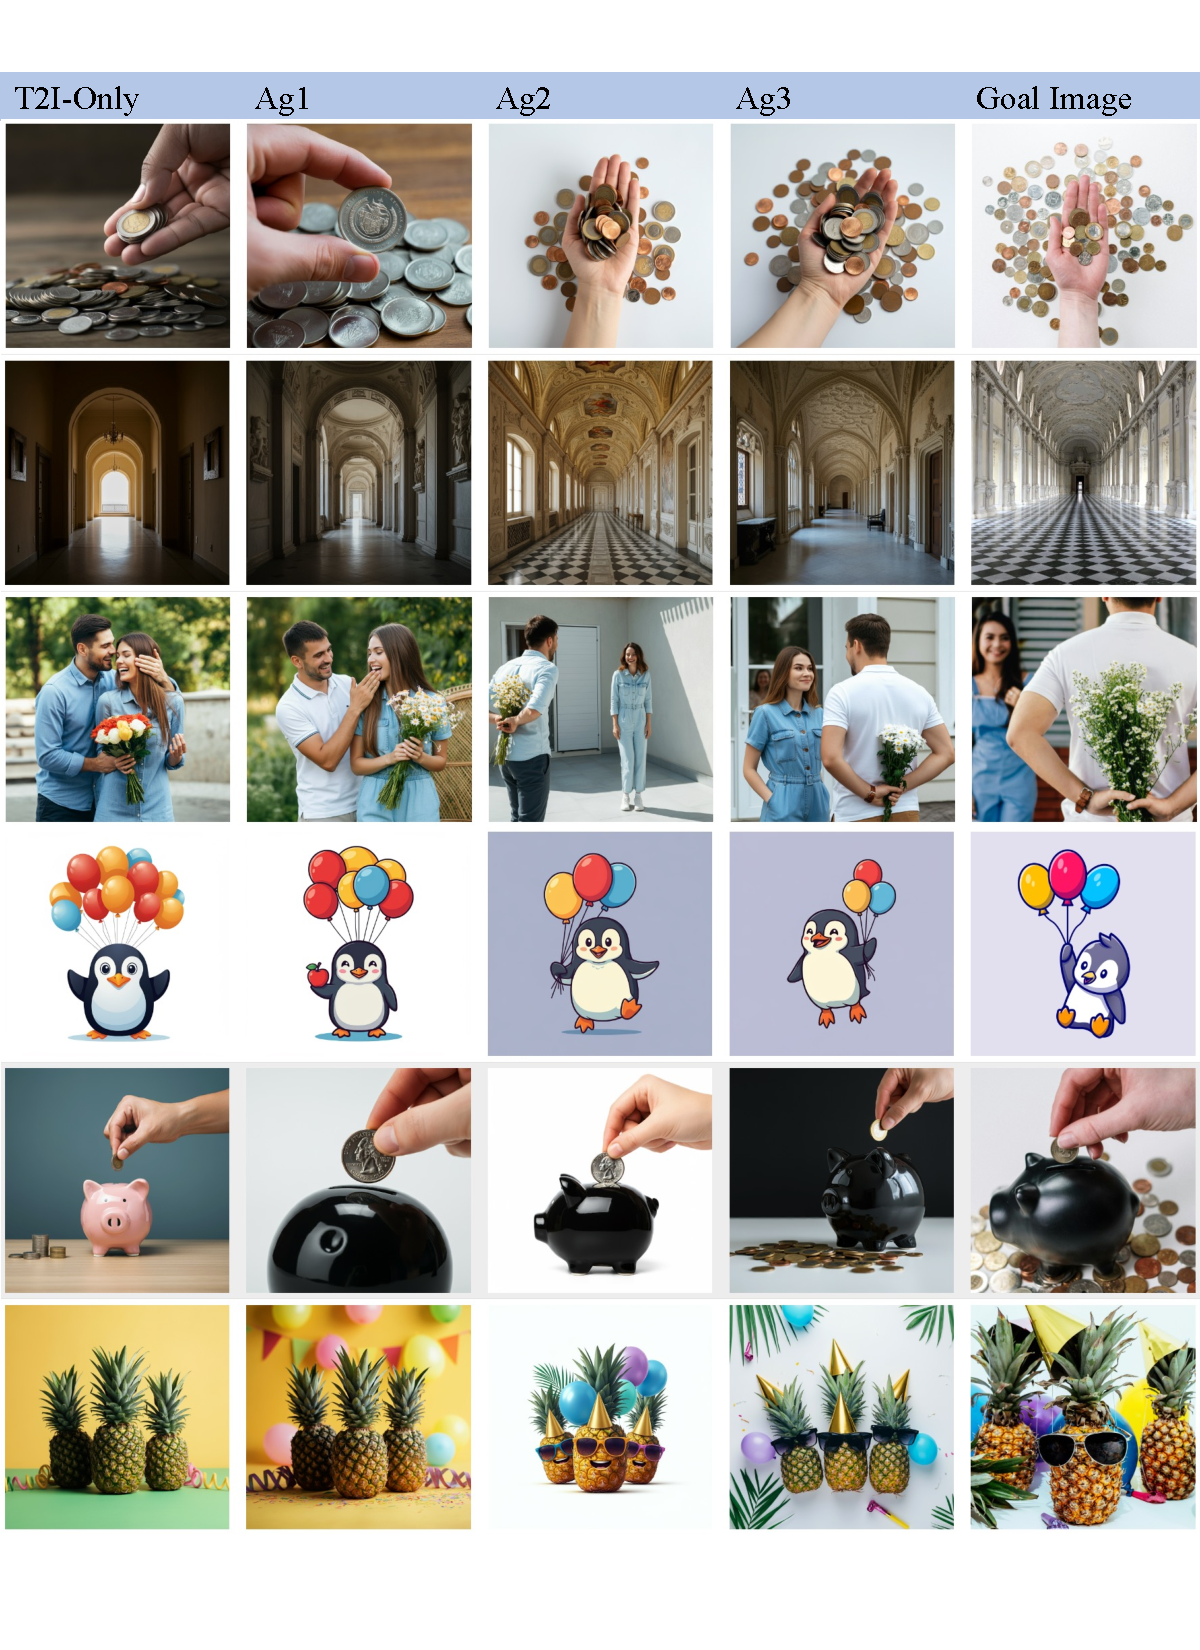
\includegraphics[width=\linewidth]{figures/toy_data_chart_part2.pdf}
    \caption{Agent Generated Image Outputs on DesignBench (Continued): a chart of the generated image outputs of the four main Agent types in comparison to the goal image. Each column displays the output of a different agent and the right most column shows the goal image that the agents aimed to recreate. Each agent was provided with the same starting prompt and iterated for 15 turns, with the exception of the "T2I" agent column which produces an image from the starting prompt. Ag1, Ag2 and Ag3 refer to the Agents described in \S \ref{ssec:implementation}. Each agent uses the same T2I model to produce the final image. The goal images displayed here are from the DesignBench dataset described in the experiments section.}
    \label{fig:toy2}
\end{figure}

\begin{figure}
    \centering
    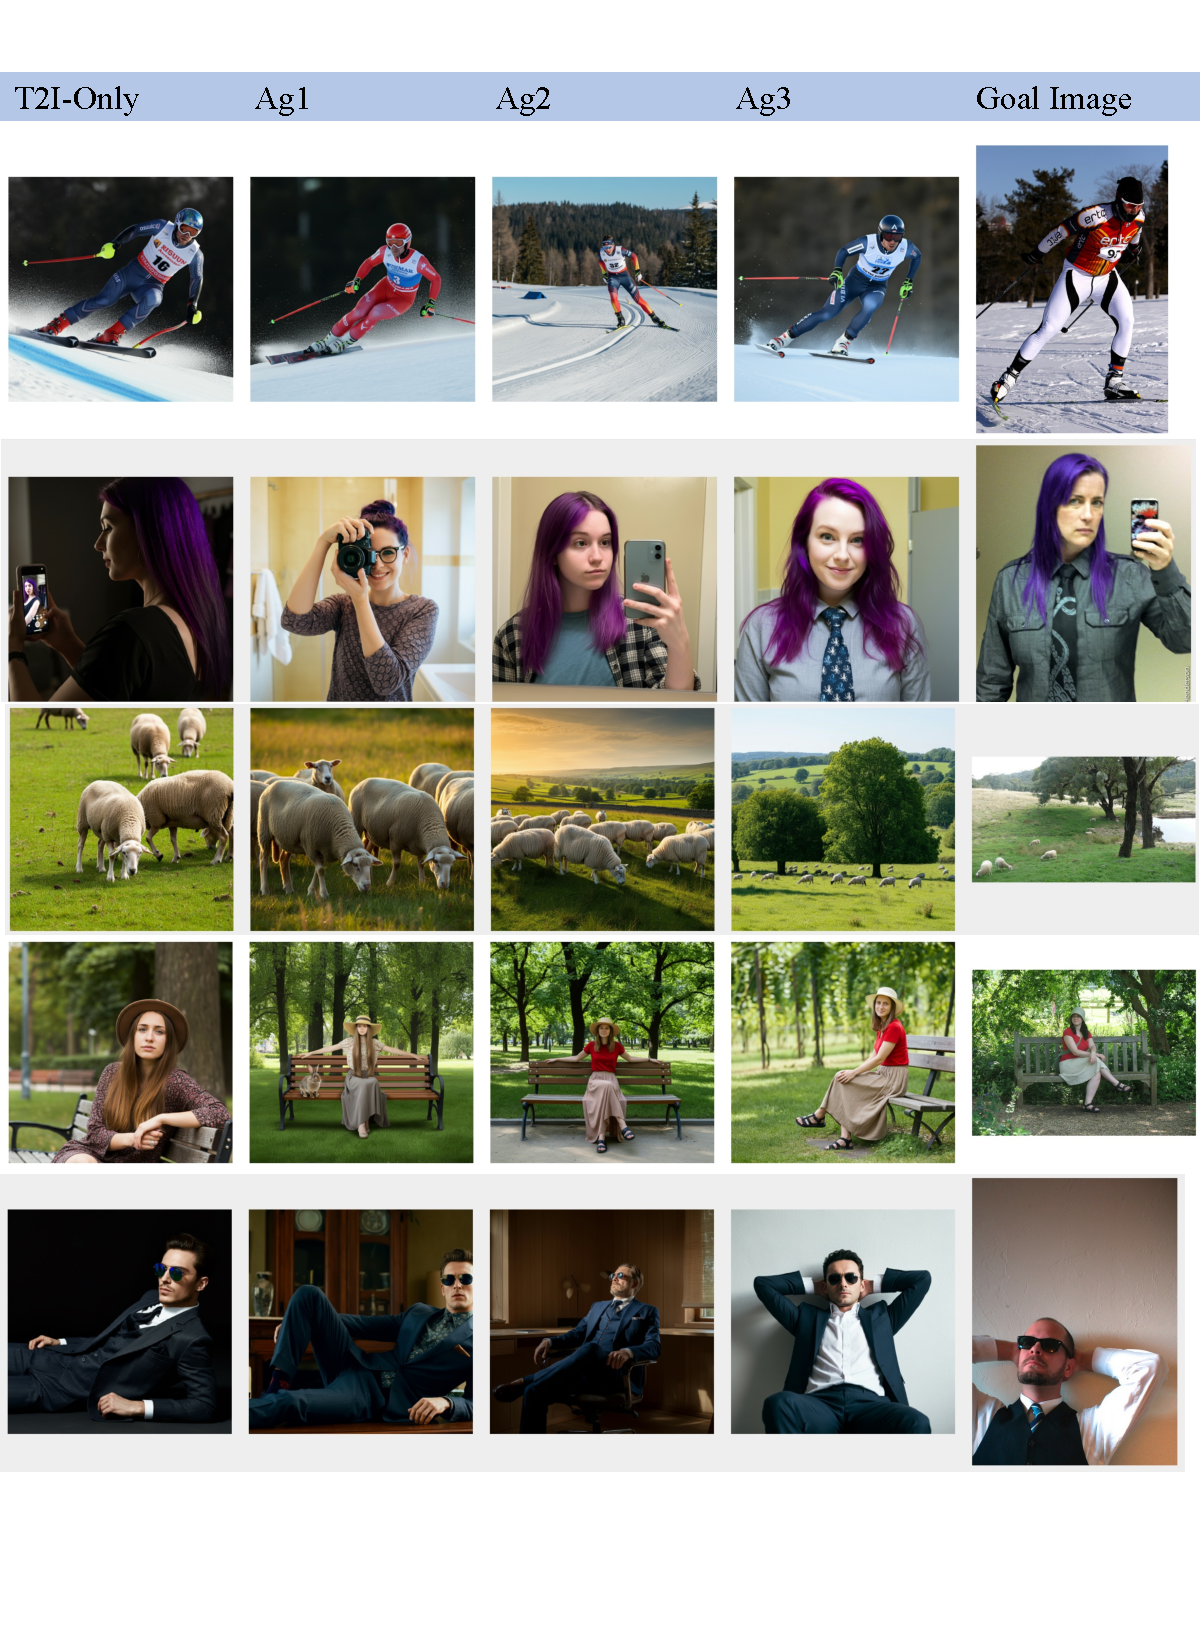
\includegraphics[width=\linewidth]{figures/coco_data_chart_part1.pdf}
    \caption{Agent Generated Image Outputs (Coco-Captions Validation): a chart of the generated image outputs of the four main Agent types in comparison to the goal image. Each column displays the output of a different agent and the right most column shows the goal image that the agents aimed to recreate. Each agent was provided with the same starting prompt and iterated for 15 turns, with the exception of the "T2I" agent column which produces an image from the starting prompt. Ag1, Ag2 and Ag3 refer to the Agents described in \S\ref{ssec:implementation}. Each agent uses the same T2I model to produce the final image. The goal images displayed here are from the Coco-Captions~\cite{chen2015microsoft} dataset described in the experiments section.}
    \label{fig:coco1}
\end{figure}

\begin{figure}
    \centering
    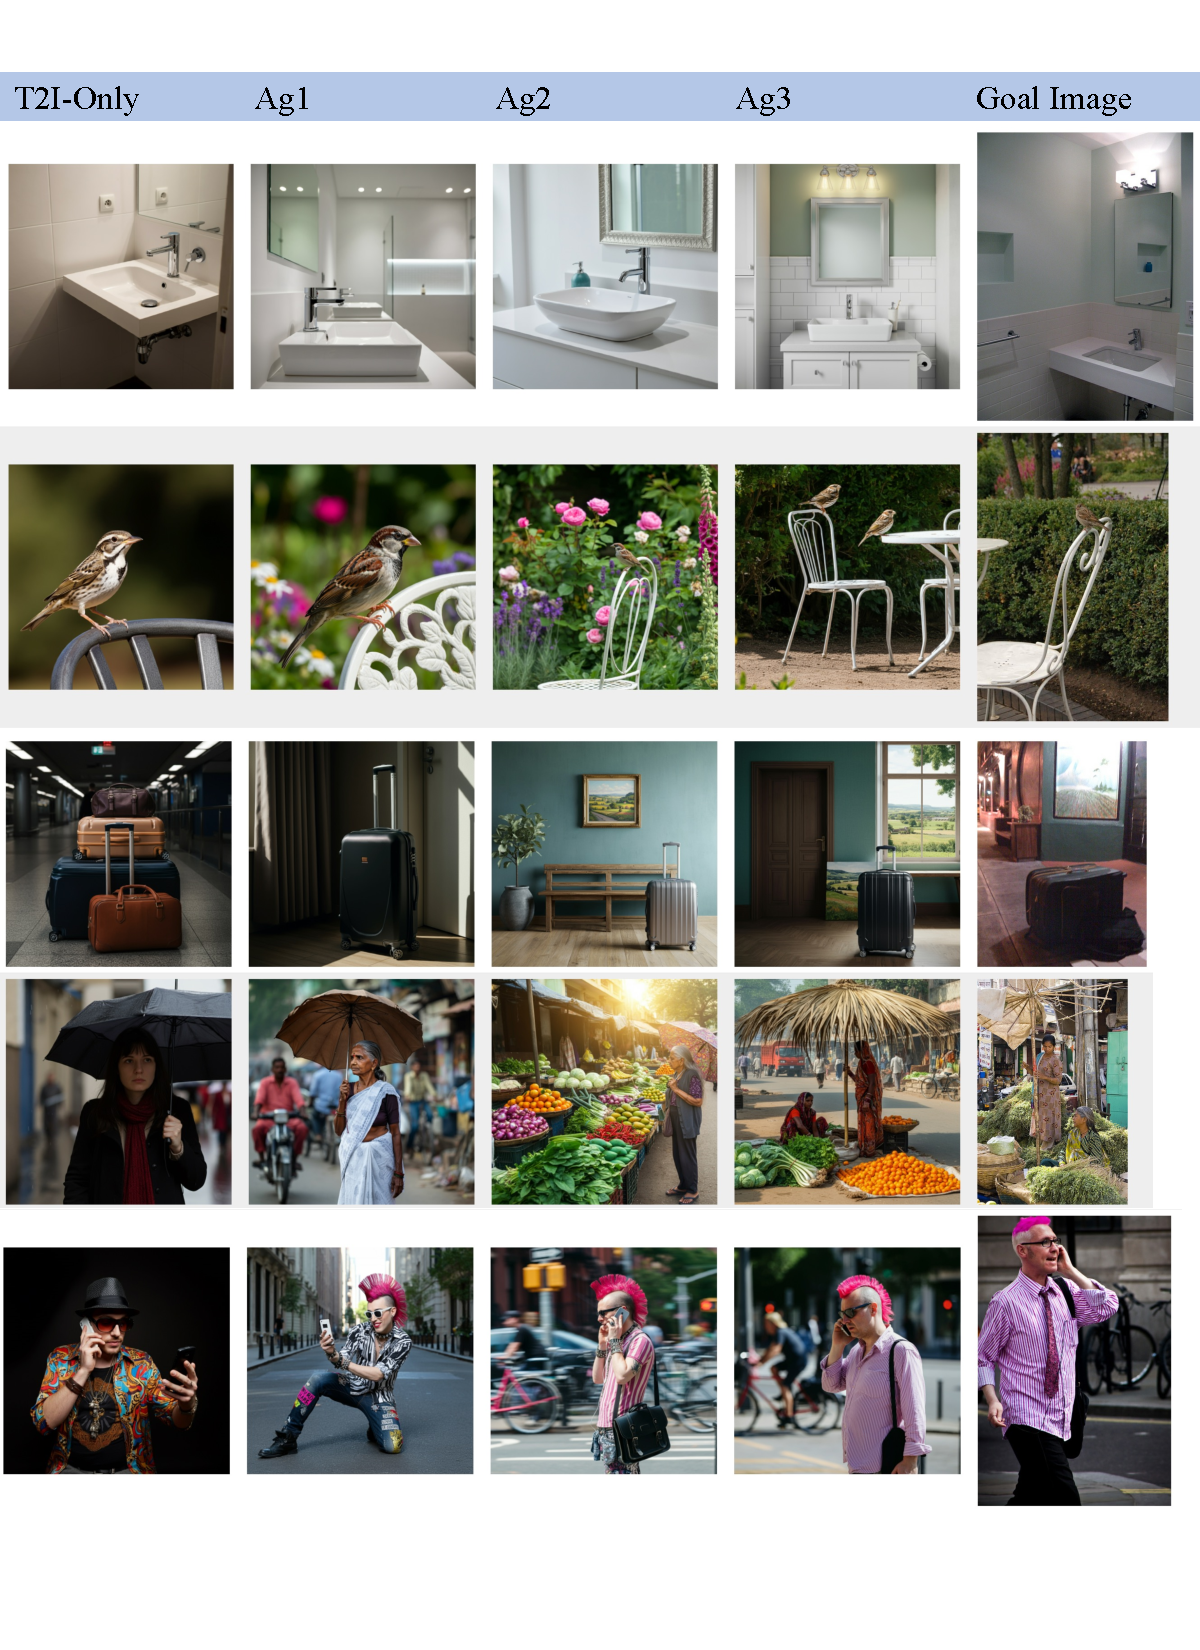
\includegraphics[width=\linewidth]{figures/coco_data_chart_part2.pdf}
    \caption{Agent Generated Image Outputs (Coco-Captions Validation): a chart of the generated image outputs of the four main Agent types in comparison to the goal image. Each column displays the output of a different agent and the right most column shows the goal image that the agents aimed to recreate. Each agent was provided with the same starting prompt and iterated for 15 turns, with the exception of the "T2I" agent column which produces an image from the starting prompt. Ag1, Ag2 and Ag3 refer to the Agent described in the methods section. Each agent uses the same T2I model to produce the final image. The goal images displayed here are from the Coco-Captions~\cite{chen2015microsoft} dataset described in the experiments section.}
    \label{fig:coco2}
\end{figure}


\section{Implementation details of agent prototypes} \label{ssec:implementation}
We propose three T2I agents, each characterized by a unique configuration of $\langle B, A, O, \tau, \pi\rangle$ tuples: 
\begin{itemize}
    \item \textit{Ag1: Heuristic Score Agent}. This agent incorporates a human-defined heuristic score based on the belief to guide question generation. This heuristic score reflects the perceived importance of different aspects of the belief in driving the conversation forward;
    \item \textit{Ag2: Belief-prompted Agent}. This agent leverages an LLM to generate questions by processing both the conversation history and a structured representation of the belief.
    \item \textit{Ag3: Principle-prompted Agent}. This agent generates questions directly from the conversation history based on the principles introduced in \S\ref{ssec:principles}. The question asking strategy of Ag3 relies solely on the implicit knowledge and reasoning capabilities of the underlying LLM.
\end{itemize}

\subsection{Implementation of agent beliefs} \label{sssec:state_implementation}



Technically, an agent belief $b\in B$ is represented in two complementary forms: (i) Merged prompt: This is a natural language representation that summarizes the entire conversation history up to the current turn. It provides a comprehensive textual overview of the user's requests, feedback, and any clarifications exchanged with the agent. (ii) Belief graph: This is a symbolic representation derived from the merged prompt. It parses the natural language text into a structured format, capturing key elements like entities, attributes, relationships, and associated probabilities. This structured representation facilitates more precise reasoning and decision-making by the agent.

\textbf{Prompt Merging.}  An LLM (\S\ref{ssec:qna_verbal}) summarizes the latest interaction, encapsulating the agent's question and the user's response into a concise textual representation. This step distills the essential information exchanged during the interaction. Another LLM (\S\ref{ssec:merge_prompt}) merges the existing merged prompt (containing the accumulated information from previous interactions) and the summarized interaction at the current turn. This creates an updated prompt that reflects the evolving understanding of the user's intent.

\textbf{Belief Parsing.} See an example of the belief graph \cref{fig:belief_state_example}. We employ three specialized parsers trained via in-context learning (ICL): entity parser (\S\ref{ssec:entity_parser}) analyzes the user prompt to identify and extract a list of relevant entities.; attribute parser (\S\ref{ssec:attribute_parser}) takes user prompt and an entity as the input to extract a list of attributes associated with that entity; relation parser (\S\ref{ssec:relation_parser}) takes the user prompt and a list of entities as input and identifies relationships between those entities. Each entity is associated with meta information like name, importance to ask score, description, probability of appearing, a list of attributes like color, position, etc \footnote{\textbf{Name} is a unique identifier for the entity; \textbf{Importance to ask score}: A numerical value indicating the entity's perceived importance in satisfying the user's request. Entities with higher scores are prioritized during question generation, as they are likely to reduce uncertainty and contribute significantly to the final image; \textbf{Description} provides a textual description of the entity; \textbf{probability of appearing} estimates likelihood of the entity being present in the generated image; \textbf{Attributes} is for understanding the detailed attributes of the entities.}. Each attribute contains meta information like name, importance to ask score, a list of possible values for the attribute along with their associated probabilities, etc. Each relation includes meta information such as: name, description, spatial relation, importance to ask score, entity 1 and entity 2, whether the relation is bidirectional, etc. 

\begin{figure}
    \centering
    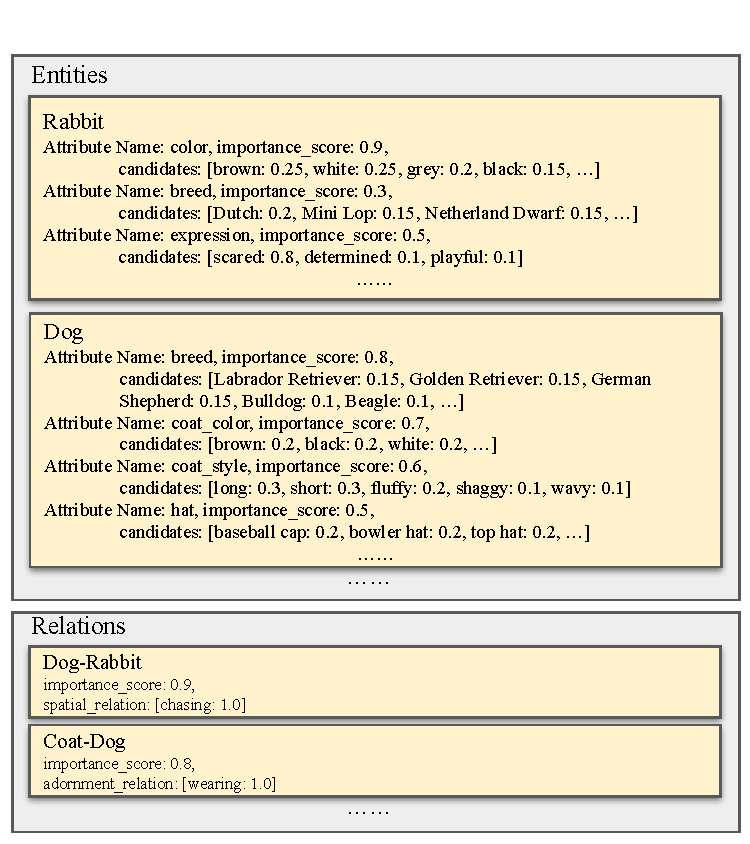
\includegraphics[width=.8\linewidth]{figures/Belief_state_visualization.pdf}
    \caption{An example of the belief graph data structure for a given prompt in \Cref{fig:first_figure_interface}.}
    \label{fig:belief_state_example}
\end{figure}


\subsection{Implementation of action} \label{sssec:action_implementation}

From an information theoretic perspective, an optimal action is the one that maximizes the information gain between the observation and the belief, i.e. $a_t = \argmax_a H(o_{i-1}; b_{i-1} \mid a) - H(o_{i}; b_{i} \mid a)$. However, directly optimizing this objective can be computationally challenging. Therefore, we explore several heuristic strategies to effectively reduce uncertainty: 
\begin{itemize}
    \item Maximize the overall heuristic importance score ($MHIS$):This strategy focuses on maximizing the overall importance score of the entities, attributes, and relations within the belief. We further ask a question regarding an attribute or relation by maximizing the overall heuristic importance score. The score can be modeled as: 

\begin{equation} \label{eq:importance_score}
max_{e, a, c, r}( IS(\text{e})*IS(\text{a})*P(\text{e})*Ent(\text{c}), IS(\text{r})*P(\text{r})*Ent(\text{c}))
\end{equation}


Here $IS, P, Ent$ represents importance to ask score, probability of appearing, and entropy of the probabilities respectively and $e, a, c, r$ represents entity, attribute, candidate list, relation respectively.
    \item Ask Important Clarification Question based on belief ($AICQ_{B}$): This strategy leverages the structured information within the belief. We provide the LLM with the user prompt, conversation history, and the current belief, utilizing an ICL prompt (\S\ref{ssec:belief_agent_prompt}) to guide question generation. The LLM then formulates a clarification question aimed at eliciting information about key features of the image, naturally prioritizing those with higher \textit{Importance to ask score} within the belief.
    \item Ask Important Clarification Question directly ($AICQ_{base}$): This strategy relies on the LLM's inherent ability to identify important aspects of the user prompt and conversation history. The LLM (\S\ref{ssec:monolithic_agent_prompt}) generates an important clarification question based on its implicit understanding of the user's needs, without explicitly relying on the structured information in the belief.
\end{itemize}

\textit{Ag1} employs $MHIS$ strategy for question generation. This strategy leverages the importance scores assigned to entities, attributes, and relations within the belief graph. It identifies the element with the highest heuristic importance score and formulates a question aimed at eliciting further information about that specific element.  The question is then verbalized using the LLM described in Section \S\ref{ssec:hsa_question}.

\textit{Ag2} utilizes the parsed belief graph as the basis for question generation. It employs the $AICQ_{B}$ strategy, which leverages the structured information within the belief graph to generate targeted clarification questions.

\textit{Ag3} relies solely on the conversation history for question generation. It employs the $AICQ_{base}$ strategy, which leverages the LLM's ability to understand the ongoing dialogue and identify key areas requiring further clarification.



\subsection{Implementation of belief transition} 
\label{sssec:transition_implementation}

 Both \textit{Ag1} and \textit{Ag2} require belief updating to incorporate new information gained during the interaction in order to compose clarification questions. At each turn, we perform prompt merging to create a comprehensive prompt that summarizes the conversation history. This merged prompt is then used for belief parsing to obtain an updated belief graph. For \textit{Ag2} (and \textit{Ag3}), this updated belief graph directly informs the subsequent interaction. For \textit{Ag1}, it incorporates additional post-processing mechanisms to enhance memory and prevent redundant questioning: (i) Redundancy elimination: If an attribute or relation has already been addressed in the conversation history, the corresponding user response is assigned as the sole candidate with a probability of 1.0, and its importance score is set to 0. This prevents the agent from repeatedly asking about the same information. (ii) Information retention: If an attribute or relation from the conversation history is absent in the updated belief graph, it is explicitly added. This ensures that the agent retains crucial information even if it's not explicitly present in the latest parsed belief graph.

\subsection{User simulation} \label{ssec:user_simulation}

To simulate end-to-end agent-user interactions, we implement a user simulator that mimics human question-answering behavior. This simulator operates as follows:
\begin{itemize}
    \item  It generates a belief graph based on a ground truth prompt, representing the user's intended image. This serves as the simulator's internal representation of the desired image.
    \item Mirroring the $AICQ_{B}$ strategy, the simulator takes the ground truth prompt, conversation history, and its current belief graph as input. It then leverages an ICL prompt (see \S\ref{ssec:belief_agent_prompt}) to generate a response to the agent's question. This ensures that the simulator's answers are consistent with its internal belief graph and the ongoing conversation.
\end{itemize}


\subsection{Ag1: Heuristic Score Agent}\label{ssec:ag1}
The \textit{Heuristic score agent} leverages the importance scores and probabilities within the belief graph to guide its question-asking strategy. The underlying principle is to identify and inquire about the entity, attribute, or relation that exhibits both high importance and high uncertainty. This aligns with the uncertainty reduction principle discussed in \S\ref{ssec:principles}, which emphasizes minimizing uncertainty through targeted questioning. To achieve this, we define a \textit{heuristic importance score} as formulated in Equation \ref{eq:importance_score}, and the agent then selects the attribute or relation with the highest heuristic importance score as the focus of its inquiry. To facilitate easy answering, we utilize an LLM to generate user-friendly questions with multiple-choice options. For example, the agent might ask: \textit{What color of the rabbit do you have in mind? a. black , b. white, c. brown. d. unkown. If none of these options , what color of the rabbit do you have in mind?}. This format allows users to simply select the most appropriate option or provide their own answer if needed. 

Here's a summary of Ag1's implementation: (i) \textbf{Belief Representation}: The agent's belief comprises the merged prompt and the current belief graph. (ii) \textbf{Select Action}: $MHIS$ strategy is employed to identify the attribute or relation of interest based on the heuristic importance score. (iii) \textbf{Verbalize Action}: An LLM (\S\ref{ssec:hsa_question}) is used to generate a clear and concise question about the selected attribute or relation. (iv) \textbf{Answer Question}: The user simulator provides an answer to the agent's question, mimicking human response behavior. (v) \textbf{Transition}: The agent updates the merged prompt with the new information, re-generates the belief graph based on the updated prompt, and applies the post-processing logic outlined in \S\ref{sssec:transition_implementation} to ensure consistency and prevent redundancy.



\subsection{Ag2: Belief-prompted Agent}\label{ssec:ag2}
The \textit{Ag2} agent incorporates the belief graph into its decision-making process but adopts a different approach compared to \textit{Ag1}. Instead of relying on a heuristic score, \textit{Ag2} leverages the full capacity of an LLM to generate questions. It provides the LLM with comprehensive information, including the merged prompt, belief graph, and conversation history, allowing the LLM to formulate the most informative questions possible. To guide the LLM towards generating effective questions, we incorporate specific instructions in the prompt, emphasizing the following principles: \textit{The question should be as concise and direct as possible. The question should aim to obtain the most information about the style, entities, attributes, spatial layout and other contents of the image. Remember to ask for information that are critical to knowing the critical details of the image that is important to the user. The question should reduce your uncertainty about the user intent as much as possible.}

Here's a summary of Ag2's implementation: (i) \textbf{Belief Representation}: The same as \textit{Ag1}, the agent's belief consists of the merged prompt and the current belief graph. (ii) \textbf{Select Action}: $AICQ_{B}$ strategy is employed, which leverages an LLM to generate a question based on the comprehensive input information. (iii) \textbf{Verbalize Action}: Since the LLM directly generates the question, no separate verbalization step is required. (iv) \textbf{Answer Question}: The user simulator provides an answer to the agent's question. (v) \textbf{Transition}: The agent updates the merged prompt with the new information and re-generates the belief graph based on the updated prompt.


\subsection{Ag3: Principle-prompted Agent}\label{ssec:ag3}
A simple and effective implementation of LLM-based multi-modal dialogue systems is to use the context to store the history of conversations between the system and the user, and directly generate the next response based on the context. %



To align with the principles outlined in \S\ref{ssec:principles}, we guide the LLM's question generation with a prompt (\S\ref{ssec:monolithic_agent_prompt}) that emphasizes all principles: \textit{Based on the original prompt and chat history please provide a question to ask about the image. The question should be as concise and direct as possible. The question should aim to learn more about the attributes and contents of the image, the objects, the spatial layout, and the style.} The prompt also includes the history of conversation. This strategy aims to generate questions that are easy for users to understand and answer, while effectively reducing the agent's uncertainty about the desired image.   

Here's a summary of Ag3's implementation: (i) \textbf{Belief Representation}: The same as \textit{Ag1} and \textit{Ag2}, the agent's belief consists of the merged prompt and the current belief graph. (ii) \textbf{Select Action}: $AICQ_{base}$ strategy is employed, which leverages an LLM to generate a question based on the conversation history. (iii) \textbf{Verbalize Action}: The LLM directly generates the question, so no separate verbalization step is needed. (iv) \textbf{Answer Question}: The user simulator provides an answer to the agent's question. (v) \textbf{Transition}: The same as \textit{Ag2}, the agent updates the merged prompt with the new information and re-generates the belief graph based on the updated prompt.


\subsection{Entity Parser Prompt Instruction} \label{ssec:entity_parser}


\lstset{
    basicstyle=\ttfamily\color{black}, 
    breaklines=true,
    columns=flexible,
    frame=single, 
    backgroundcolor=\color{gray!5},
    keywordstyle=\color{magenta},
    showstringspaces=false,
    tabsize=2,
    numbersep=5pt, 
    numbers=left, 
    keepspaces=true, 
    breakatwhitespace=false,
    stringstyle=\color{codepurple}
}


\begin{lstlisting}[
    basicstyle=\tiny
]
Given a text-to-image prompt list out all the entities that are mentioned in the prompt. 

**Explicit Entities:** List all clearly stated entities within the prompt (people, objects, animals, locations, etc.).
**Implicit Entities:** Identify potential entities that are implied or strongly suggested by the prompt, even if not explicitly mentioned. 
**Background Entities:** Deduce relevant background elements which could impact the image generation from the prompt or context, including:
    **Weather:** If the scene or mood suggests specific weather conditions (sunny, rainy, stormy, etc.).
    **Location:** If a general or specific setting is hinted at (indoors, outdoors, a particular city/landscape, etc.).
    **Time of Day:** If the prompt implies a certain time (dawn, midday, dusk, night).
    **Mood or Atmosphere:** If the prompt evokes a particular emotion or ambiance (joyful, mysterious, peaceful, etc.).


The output should be list and each entry should be formated as a JSON dict with the following fields:

"name": The name of the entity.
"importance_to_ask_score": The importance score of asking a question about this entity to reduce the uncertainty of what the image is given the user prompt. Make sure that this is a number between 0 and 1, higher means more important. Consider these factors when assigning scores: 1. Increate the score for entities that are the primary focus or subject of the prompt; 2. increase the score for entities that could strongly influence the layout of the image, such as the position or portrayal of other entities in the scene; 3. significantlydescrease the score for entities that are already well specified in the prompt; 4. significantlyincrease the score for implicit entities that are likely to appear in the image and their appearance can significantly impact the image.
"description": A short description of the entity.
"entity_type": The type of this entitiy. It could be either explicit, implicit, background. No other value is allowed.
"probability_of_appearing": The probability of the entity appearing in the image. This is a number between 0 and 1. You should assign a probability with the following rules in mind:
  1. If the prompt says an entity does not exist, assign a 0.0 probability. Because the entity does not exist, you should also assign 0 to importance_to_ask_score of this entity.
  2. If the prompt indicates an entity definitly exists in the image, assign a 1.0 probability.
  3. If the prompt does not say anything about the existence of the entity, assign a probability between 0 and 1. This probability is higher if the entity is more likely to appear in the image given the context specified by the prompt.
  4. If the prompt says an entity exists but there is an indication that the entity is not likely to appear in the image, assign a probability between 0 and 1, higher if the entity is more likely to appear in the image.

Below is an example input and output pair:
Example1:
Input: {{
  "user_prompt": "generate an image of a lionhead rabbit running on grass with sun shining. There is no trees in the background."
}}
Output: [
    {{
      "name": "rabbit",
      "importance_to_ask_score": 0.5,
      "description": "a lionhead rabbit",
      "entity_type": "explicit",
      "probability_of_appearing": 1.0
    }},
    {{
      "name": "grass",
      "importance_to_ask_score": 0.5,
      "description": "grass",
      "entity_type": "explicit",
      "probability_of_appearing": 1.0
    }},
    {{
      "name": "sun",
      "importance_to_ask_score": 0.1,
      "description": "sun is shining",
      "entity_type": "explicit",
      "probability_of_appearing": 0.3
    }},
    {{
      "name": "sun light",
      "importance_to_ask_score": 0.1,
      "description": "sun light shining on the grass and the rabbit",
      "entity_type": "explicit",
      "probability_of_appearing": 1.0
    }},
    {{
      "name": "tree",
      "importance_to_ask_score": 0,
      "description": "trees in the background",
      "entity_type": "explicit",
      "probability_of_appearing": 0
    }}
    {{
      "name": "camera angle",
      "importance_to_ask_score": 0.8,
      "description": "the camera angle of the image",
      "entity_type": "background",
      "probability_of_appearing": 1.0
    }},
    {{
      "name": "weather",
      "importance_to_ask_score": 0.8,
      "description": "weather",
      "entity_type": "background",
      "probability_of_appearing": 1.0
    }},
    {{
      "name": "image style",
      "importance_to_ask_score": 1.0,
      "description": "the style of the image",
      "entity_type": "background",
      "probability_of_appearing": 1.0
    }},
    {{
      "name": "background color",
      "importance_to_ask_score": 0.8,
      "description": "the background color of the image",
      "entity_type": "background",
      "probability_of_appearing": 0.5
    }}
]

... [[a few additional examples]] ...


Identify the entities given the input given below. Strictly stick to the format.
Input: {{
  "user_prompt": "{user_prompt}"
}}
Output: 
\end{lstlisting}

\subsection{Attribute Parser Prompt Instruction} \label{ssec:attribute_parser}
\begin{lstlisting}[
    basicstyle=\tiny, %
]
Given a text-to-image prompt and a particular entity described in the prompt, and your goal is to identify a list possible attributes that could describe the particular entity. Output Requirements:

1. if this attribute has already existed as an entity in other existing entity list, then do not include it. 
2. the attribute candidate could be a mixed of values like `color A and color B`.
3. The output should be a json parse-able format:

name (str): The name of the attribute.
importance_to_ask_score (float): The importance score of asking a question about this attribute to reduce the uncertainty of what the image is given the user prompt. This is a number between 0 and 1, higher means more important. Consider these factors when assigning scores: 1. Increate the score for attributes that are the primary attributes of an important entity; 2. significantly increase the score for attributes that could strongly influence the generation or portrayal of OTHER attributes in the scene; 3. descrease the score for attributes that are already well specified in the prompt. For example, a breed of a dog would impact other attributes like color, size, etc. So the breed attribute should have a higher importance score than color, size, etc. Assign a much lower score if the attribute's value is already mentioned in the user prompt.
candidates (List of names and probabilities): List of possible values that the attribute can take. Make sure to generate atleast 5 or more possible values. These should be realistic for the given entity. For each attribute, returns the probability that the user wants this candidate based on the user prompt. If it's already mentioned by the user, only generate one candidate (the mentioned one) and assign 1.0 as the probability. The sum of probabilities over all candidates shall be 1. Also infer the probability based on the prompt. For example, for a dog with breed Samoyed, the color attribute has a very high probability of white.

Below are two examples of input and output pairs:

Example 1:
Input: {{
  "user_prompt": "generate an image of a white rabbit running on grass",
  "entity": "rabbit",
  "other_existing_entities": "grass"
}}
Output: [
    {{
      "name": "color",
      "importance_to_ask_score": 0.9,
      "candidates": {{"white":1.0}}
    }},
    {{
      "name": "breed",
      "importance_to_ask_score": 1.0,
      "candidates": {{"Dutch": 0.20,
                    "Mini Lop": 0.15,
                    "Netherland Dwarf": 0.15,
                    "Lionhead": 0.10,
                    "Flemish Giant": 0.10,
                    "Mini Rex": 0.10,
                    "English Angora": 0.08,
                    "Mini Satin": 0.05,
                    "Himalayan": 0.05,
                    "Californian": 0.02}}
    }},
    {{
      "name": "age",
      "importance_to_ask_score": 0.1,
      "candidates": {{"adult": 0.6,
                      "baby": 0.2,
                      "senior": 0.2}}
    }}
  ]

... [[a few additional examples]] ...

Generate attributes given the input given below. Do not include other entities in the attributes. Strictly stick to the format.
Input: {{
  "user_prompt": "{user_prompt}",
  "entity": "{entity.name}",
  "other_existing_entities": "{existing_entities}"
}}
Output: 
\end{lstlisting}

\subsection{Relation Parse Prompt Instruction} \label{ssec:relation_parser}
\begin{lstlisting}[
    basicstyle=\tiny, %
]
Given a text-to-image prompt and a list of entity described in the prompt, your goal is to identify a list of entity pairs that have relations between them. Ignore entity pairs without relations. The output should be a json parse-able format (No comma after the last element of the list):

Input:
user_prompt: the prompt from the user.
entities: a list of entities mentioned in the user_prompt.

Output:
name (str): The name of the relation. Use `entity1-entity2` as the format.
description (str): A short description of the relation.
spatial_relation (map from potential relation candidates to probability): Possible spatial relations between the two entities. If a relation is mentioned in the user prompt, assign 1.0 as the probability. The sum of probabilities over all relation candidates shall be 1.
importance_to_ask_score (float): The importance score of asking a question regarding this relation to reduce entropy. This is a number between 0 and 1, higher means more important. Assign a higher score if the two entities are very important, the relation between them is very unclear, and the relation is very important for the layout of the image.
name_entity_1 (str): The name of the first entity.
name_entity_2 (str): The name of the second entity.
is_bidirectional (bool): Whether the relation is bidirectional.

Below is an example input and output pair:
Example1:
Input: {{
  "user_prompt": "generate an image of a lionhead rabbit sitting on grass, and a eagle is flying through the sky. There is a tree in the background.",
  "entity": ["rabbit", "grass", "eagle", "tree"]
}}
Output: [
    {{
      "name": "rabbit-grass",
      "description": "rabbit sitting on grass",
      "spatial_relation": {{"above": 0.8, "below": 0.0, "in front of": 0.0, "behind": 0.0, "left of": 0.1, "right of": 0.1}},
      "importance_to_ask_score": 0.1,
      "name_entity_1":"rabbit",
      "name_entity_2": "grass",
      "is_bidirectional": true
    }},
    {{
      "name": "eagle-grass",
      "description": "eagle is flying through the sky",
      "spatial_relation": {{"above": 1.0, "below": 0.0, "in front of": 0.0, "behind": 0.0,"left of": 0.0, "right of": 0.0}},
      "importance_to_ask_score": 0.1,
      "name_entity_1":"eagle",
      "name_entity_2": "grass",
      "is_bidirectional": false
    }},
    {{
      "name": "tree-grass",
      "description": "",
      "spatial_relation": {{"above": 0.5, "below": 0.0, "in front of": 0.0, "behind": 0.0, "left of": 0.25, "right of": 0.25}},
      "importance_to_ask_score": 0.1,
      "name_entity_1":"tree",
      "name_entity_2": "grass",
      "is_bidirectional": false
    }},

    ... [[a few additional examples]] ...

  ]

Identify relationships between entities given the input given below. Strictly stick to the format.
Input: {{
  "user_prompt": "{user_prompt}",
  "entity": "{entity_names}"
}}
Output: 
\end{lstlisting}

\subsection{Verbalization Prompt Instruction} \label{ssec:qna_verbal}
\begin{lstlisting}[
    basicstyle=\tiny, %
]
The chat history is as follows:
question: {action.verbalized_action} and answer: {observation}.
Turn the question and action into a single declarative sentence that describes the answer - do not phrase it as a question. Example output: the firetruck in the image is red.
\end{lstlisting}

\subsection{Merge Prompt Prompt Instruction} \label{ssec:merge_prompt}
\begin{lstlisting}[
    basicstyle=\tiny, %
]
You are writing a prompt for a text-to-image model based on user feedback. The original prompt is {prompt}. The user has provided some additional information: {additional_info}. Please write a new prompt for the text-to-image model. The new prompt should be a meaningful sentence or a paragraph that combines the original prompt and the additional information. Do not add any new information that is not mentioned in the prompt or the additional information. Make sure the information in the original prompt is not changed. Make sure the additional information is included in the new prompt. Make sure the new prompt is a description of an image. If the additional information or the original prompt specifically says that a thing does not exist in the image, you should make sure the new prompt mentions that this thing does not exist in the image. DO NOT generate rationale or anything that is not part of a description of the image.
\end{lstlisting}

\subsection{$AICQ_{base}$ Prompt Instruction} \label{ssec:monolithic_agent_prompt}

\begin{lstlisting}[
    basicstyle=\tiny, %
]
... [[Instruction for the first question]] ...

The original prompt was: {self.original_prompt} - Based on the original prompt please provide a question to ask about the image. The question should be as concise and direct as possible. The question should aim to learn more about the attributes and contents of the image, the objects, the spatial layout, and the style. Make sure that you question the answer within <question> and </question> markers

... [[Instruction for the following question]] ...

Based on the chat history please provide a new question to ask about the image. the chat history is as follows and is enclosed in  <chat_history> and </chat_history> markers:{self.chat_history} </chat_history> The question should be as concise and direct as possible. The question should aim to learn more about the attributes and contents of the image, the objects, the spatial layout, and the style. Make sure that you question the answer within <question> and </question> markers.'
\end{lstlisting}

\subsection{$AICQ_{B}$ Prompt Instruction} \label{ssec:belief_agent_prompt}

\begin{lstlisting}[
    basicstyle=\tiny, %
]
You are an intelligent agent that helps users generate images. Before generating the image requested by the user, you should ask the most important clarification questions to make sure you understand the key features of the image. 
The user describes the image as: {user_prompt}.
The following is your belief of what the image contains, including the entities, attributes of each entity and relations between entities. 
Each entity has "name", "descriptions", "importance to ask score" and  "probability of appearing". "Name" is the identifier of the entity. "Descriptions" is the description of the entity. "Importance to ask score" is how important it is for the agent to ask whether the entity exists. Probability of appearing" is the probability the agent estimated that this entity exits in the image.

Each entity has a list of attributes. Each attribute has "name", "importance to ask score" and "candidates". "Name" is the identifier of the attribute. "Importance to ask score" is how important it is to ask about the exact value for the attribute of the entity. "Candidates" is a list of possible values for the attribute.

Each candidate value has a probability that describes how likely this candidate value should be assigned to the attribute. 
For example, "Attribute Name: color, Importance to ask Score: 0.9, Candidates: [white: 0.5, black: 0.5]" means the color is either white or black, each with 0.5 probability. If you ask about attributes, you should ask about the attribute with the highest uncertainty. Your uncertainty can be judged by the probabilities. If the probabilities are 0.5 and 0.5, you are uncertain. If the probabilities are 0.1 and 0.9, you are fairly certain. 

The agent belief is:
{belief_state.__str__()} 

Based on the user prompt "{user_prompt}" and the belief of the agent, please provide a question to ask about the image. The question should be as concise and direct as possible. The question should aim to obtain the most information about the style, entities, attributes, spatial layout and other contents of the image. Remember to ask for information that are critical to knowing the critical details of the image that is important to the user. The question should reduce your uncertainty about the user intent as much as possible. DO NOT ask question that can be answered by common sense. DO NOT ask question that are obvious to answer based on the user prompt "{user_prompt}". DO NOT ask any question about information present in the following user-agent dialogue within <dialogue> and </dialogue> markers. 

<dialogue>
{conversation}
</dialogue>

DO NOT ask any question that has been asked in the dialogue above.

Your question does not have to be entirely decided by the belief. You can construct any question that make yourself more confident about what the image is. 
Think step by step and reason about your uncertainty of the image to generate. Make sure to ask only one question. Make sure it is not very difficult for the user to answer. For example, do not ask a very very long question, which can take the user a long time to read and answer.
Make sure that you question the answer within <question> and </question> markers. 
\end{lstlisting}


\subsection{HSA Question Prompt Instruction} \label{ssec:hsa_question}
\begin{lstlisting}[
    basicstyle=\tiny, %
]
You are constructing a text-to-image (T2I) prompt and want more details from the user.
You have to ask a question about the the most important entity or the attribute of the most important entity.
We have entity types: (i) explicit: directly ask question with options; (ii) implicit: ask whether this entity required for the image with yes or no as options; (iii) background: ignore the attribute value and directly ask the value of the entity. (iv) relation: add keyword like `relation` to emphasize this entity is a relation.
Construct a simple question that directly asks this information from the user and also provides option that the user can pick from. Ask only one question and follow it with options.


Example1:
entity: rabbit
attribute: color
candidates: black, white, brown
entity_type: explicit
question: What color of the rabbit do you have in mind? a. black, b. white, c. brown. d. unkown. If none of these options, what color of the rabbit do you have in mind?

... [[a few additional examples]] ...

Example5:
entity: $entity
attribute: $attribute
candidates: $candidates
entity_type: $entity_type
question: 
\end{lstlisting}





